\PassOptionsToPackage{no-math,cm-default}{fontspec}
\documentclass[twoside,nofonts,internet,shmeiwseis]{thewria}
\usepackage{amsmath}
\usepackage{xgreek}
\let\hbar\relax
\defaultfontfeatures{Mapping=tex-text,Scale=MatchLowercase}
\setmainfont[Mapping=tex-text,Numbers=Lining,Scale=1.0,BoldFont={Minion Pro Bold}]{Minion Pro}
\newfontfamily\scfont{GFS Artemisia}
\font\icon = "Webdings"
\usepackage[amsbb]{mtpro2}
\usepackage{tikz,pgfplots}
\tkzSetUpPoint[size=7,fill=white]
\xroma{red!70!black}


\newlist{rlist}{enumerate}{3}
\setlist[rlist]{itemsep=0mm,label=\textcolor{\xrwma}{\roman*.}}
\newlist{brlist}{enumerate}{3}
\setlist[brlist]{itemsep=0mm,label=\bf\roman*.}
\newlist{tropos}{enumerate}{3}
\setlist[tropos]{label=\bf\textit{\arabic*\textsuperscript{oς}\;Τρόπος :},leftmargin=0cm,itemindent=2.3cm,ref=\bf{\arabic*\textsuperscript{oς}\;Τρόπος}}
\newcommand{\tss}[1]{\textsuperscript{#1}}
\newcommand{\tssL}[1]{\MakeLowercase{\textsuperscript{#1}}}

\usepackage{hhline}
\usepackage{gensymb}
\setlist[enumerate]{label=\bf{\large{\textcolor{\xrwma}{\arabic*.}}}}
\usepackage{multicol}
\usepackage{wrap-rl}
\usepackage{mathimatika}

\begin{document}
\titlos{ΜΑΘΗΜΑΤΙΚΑ ΚΑΤΕΥΘΥΝΣΗΣ Β΄ ΛΥΚΕΙΟΥ}{ΔΙΑΝΥΣΜΑΤΑ}{Πρόσθεση και αφαίρεση διανυσματων}
\orismoi
\Orismos{Πρόσθεση διανυσμάτων - Διαδοχικά διανύσματα}
Άθροισμα ή συνισταμένη δύο μη μηδενικών \textbf{διαδοχικών}  διανυσμάτων $ \vec{a} $ και $ \vec{\beta} $ ονομάζεται το διάνυσμα $ \vec{a}+\vec{\beta} $ το οποίο έχει αρχή, την αρχή του $ \vec{a} $ και πέρας, το πέρας του $ \vec{\beta} $.
\begin{center}
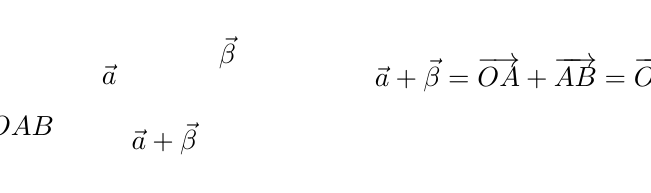
\begin{tikzpicture}
\dianysma{0,0}{1.5,1}{A}{B}
\dianysma{1.5,1}{2.7,.5}{C}{D}
\tkzLabelPoint[above](A){$O$}
\tkzLabelPoint[above](B){$A$}
\tkzLabelPoint[right](D){$B$}
\dianysma{0,0}{2.7,.5}{E}{Z}
\node at (.7,.77){$\vec{a}$};
\node at (2.2,1.04){$\vec{\beta}$};
\node at (1.4,-.05){$\vec{a}+\vec{\beta}$};
\node at (6,.77){$\vec{a}+\vec{\beta}=\overrightarrow{OA}+\overrightarrow{AB}=\overrightarrow{OB}$};
\end{tikzpicture}
\end{center}
\begin{itemize}[itemsep=0mm]
\item Αν τα διανύσματα $ \vec{a} $ και $ \vec{\beta} $ δεν είναι διαδοχικά τότε μεταφέρουμε παράλληλα ένα εκ των δύο ώστε η αρχή του να συμπέσει με το πέρας του πρώτου.
\item Το άθροισμα των διανυσμάτων είναι ανεξάρτητο από την επιλογή της αρχής $ O $.
\end{itemize}
\Orismos{Πρόσθεση διανυσμάτων - Κανόνας Παραλληλογράμμου}
Άθροισμα ή συνισταμένη δύο μη μηδενικών διανυσμάτων $ \vec{a}=\overrightarrow{OA} $ και $ \vec{\beta}=\overrightarrow{OB} $ που έχουν \textbf{κοινή αρχή}, ονομάζεται το διάνυσμα $ \vec{a}+\vec{\beta}=\overrightarrow{OM} $ το οποίο αποτελεί τη \textbf{διαγώνιο} του παραλληλογράμμου $ OAMB $ που ορίζουν οι διαδοχικές πλευρές $ OA $ και $ OB $.
\begin{center}
\begin{tikzpicture}
\dianysma{0,0}{1,1.5}{A}{B}
\dianysma{0,0}{2.4,0}{C}{D}
\dianysma{0,0}{3.4,1.5}{E}{Z}
\draw[dashed] (2.4,0)--(3.4,1.5);
\draw[dashed] (1,1.5)--(3.4,1.5);
\tkzLabelPoint[left](A){$O$}
\tkzLabelPoint[above](B){$A$}
\tkzLabelPoint[right](D){$B$}
\tkzLabelPoint[right,yshift=1mm](Z){$M$}
\node at (.2,.77){$\vec{a}$};
\node at (1.2,-.33){$\vec{\beta}$};
\node[rotate=23.8] at (1.4,.9){$\vec{a}+\vec{\beta}$};
\node at (6,.77){$\vec{a}+\vec{\beta}=\overrightarrow{OA}+\overrightarrow{OB}=\overrightarrow{OM}$};
\end{tikzpicture}
\end{center}
\Orismos{Αφαίρεση διανυσμάτων}
Η διαφορά $ \vec{a}-\vec{\beta} $ δύο μη μηδενικών διανυσμάτων $ \vec{a} $ και $ \vec{\beta} $ ορίζεται ως το άθροισμα του διανύσματος $ \vec{a} $ με το αντίθετο του $ \vec{\beta} $.
\begin{center}
\begin{tikzpicture}
\dianysma{0,0}{1.5,1}{A}{B}
\dianysma{1.5,1}{2.7,.5}{C}{D}
\tkzLabelPoint[above](A){$O$}
\tkzLabelPoint[above](B){$B$}
\tkzLabelPoint[right](D){$A$}
\dianysma{0,0}{2.7,.5}{E}{Z}
\node at (.7,.77){$\vec{a}$};
\node at (2.2,1.04){$-\vec{\beta}$};
\node at (1.4,-.05){$\vec{a}-\vec{\beta}$};
\node at (4,-1){$\vec{a}-\vec{\beta}=\vec{a}+\left( -\vec{\beta}\right)$};
\dianysma{5,0}{6,1.5}{K}{L}
\dianysma{5,0}{7.4,0}{M}{N}
\dianysma{6,1.5}{7.4,0}{O}{P}
\draw[dashed] (7.4,0)--(8.4,1.5);
\draw[dashed] (6,1.5)--(8.4,1.5)node[xshift=2mm,yshift=2mm](S){$M$};
\tkzLabelPoint[left](K){$O$}
\tkzLabelPoint[above](L){$A$}
\tkzLabelPoint[right](N){$B$}
\node at (5.2,.77){$\vec{a}$};
\node at (6.2,-.33){$\vec{\beta}$};
\node[rotate=-49] at (7.1,.77){$\vec{a}-\vec{\beta}$};
\end{tikzpicture}
\end{center}
\begin{itemize}[itemsep=0mm]
\item Με τον κανόνα της πρόσθεσης διαδοχικών διανυσμάτων τοποθετούμε στο πέρας του $ \vec{a} $ την αρχή του διανύσματος $ -\vec{\beta} $.
\item Με τον κανόνα του παραλληλογράμμου η διαφορά των δύο διανυσμάτων $ \vec{a}=\overrightarrow{OA} $ και $ \vec{\beta}=\overrightarrow{OB} $ ορίζεται ως η δεύτερη διαγώνιος $ \overrightarrow{AB} $ του παραλληλογράμμου $ OAMB $. Έχει αρχή το πέρας του $ \vec{a} $ και πέρας, το πέρας του $ \vec{\beta} $.
\end{itemize}
\Orismos{Διάνυσμα Θέσης}
Διάνυσμα θέσης ή διανυσματική ακτίνα ενός σημείου $ M $ ονομάζεται το διάνυσμα $ \overrightarrow{OM} $ με αρχή ένα τυχαίο σταθερό σημείο $ O $ του επιπέδου και πέρας το σημείο $ M $.
\begin{itemize}[itemsep=0mm]
\item Το σταθερό σημείο $ O $ ονομάζεται \textbf{σημείο αναφοράς}.
\item Το σημείο $ O $ είναι αρχή όλων των διανυσματικ΄ων ακτίνων του ίδιου επιπέδου ή χώρου και η επιλογή του είναι αυθαίρετη.
\end{itemize}
\thewrhmata
\Thewrhma{Ιδιότητες πρόσθεσης διανυσμάτων}
Στον παρακάτω πίνακα φαίνονται οι ιδιότητες της πράξης της πρόσθεσης διανυσμάτων.\\
\begin{center}
\begin{tabular}{cc}
\hline \rule[-2ex]{0pt}{5.5ex} \textbf{Ιδιότητα} & \textbf{Συνθήκη}  \\ 
\hhline{==} \rule[-2ex]{0pt}{5.5ex} Αντιμεταθετική & $ \vec{a}+\vec{\beta}=\vec{\beta}+\vec{a} $  \\ 
 \rule[-2ex]{0pt}{5.5ex} Προσεταιριστική & $ \vec{a}+\left( \vec{\beta}+\vec{\gamma}\right) =\left( \vec{a}+\vec{\beta}\right) +\vec{\gamma} $  \\ 
 \rule[-2ex]{0pt}{5.5ex} Ουδέτερο στοιχείο & $ \vec{a}+\vec{0}=\vec{a} $  \\ 
  \rule[-2ex]{0pt}{5.5ex} Αντίθετα διανύσματα & $ \vec{a}+(-\vec{a})=\vec{0} $  \\
\hline 
\end{tabular}
\end{center}
\vspace{3mm}
\Thewrhma{Διάνυσμα θέσης}
Κάθε διάνυσμα $ \overrightarrow{AB} $ του επιπέδου ή του χώρου γράφεται ως η διαφορά της διανυσματικής ακτίνας του πέρατος $ \overrightarrow{OB} $ με τη διανυσματική ακτίνα της αρχής $ \overrightarrow{OA} $.
\[ \overrightarrow{AB}=\overrightarrow{OB}-\overrightarrow{OA} \]
\Thewrhma{Μέτρο αθροίσματος διανυσμάτων}
Το μέτρο του αθροίσματος δύο μη μηδενικών διανυσμάτων $ \vec{a} $ και $ \vec{\beta} $ είναι μικρότερο ίσο από το άθροισμα των μέτρων τους και μεγαλύτερο ίσο από τη διαφορά τους.
\[ \left||\vec{a}|-|\vec{\beta}| \right| \leq\left|\vec{a}+\vec{\beta}\right|\leq|\vec{a}|+|\vec{\beta}|  \]
\end{document}
